\subsection{Naive Bayes Optimization}

The timing was measured with different bin sizes. 
In figure \ref{fig:baye_timing} the timing and success can be seen.
The timing is linear and there is no increase in successful classifications with more than 100 bins. 
The time it took to normalize the data into bins and calculate the naive Bayes is shown.

\begin{figure}[H]
\centering
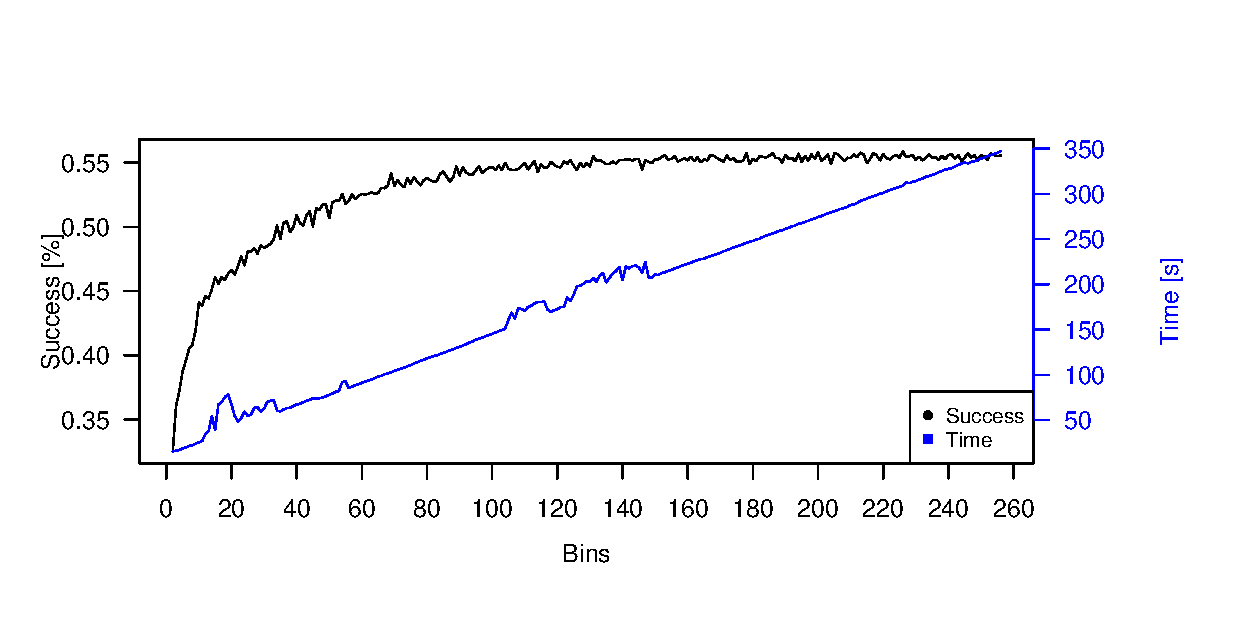
\includegraphics[width = \textwidth]{graphics/baye_timing_bins}
\caption[Timing with different bin sizes]{Timing and success of different bin sizes. Data was tested on Group 3 member 2's data vs 16 people.}
\label{fig:baye_timing}
\end{figure}


The best values for bins and PCA are taken from figure \ref{fig:contour_bin-vs-pca} and then used to compare every person with the rest of the class as seen in figure \ref{fig:comp_naiveBayes}.

\begin{figure}[H]
\centering
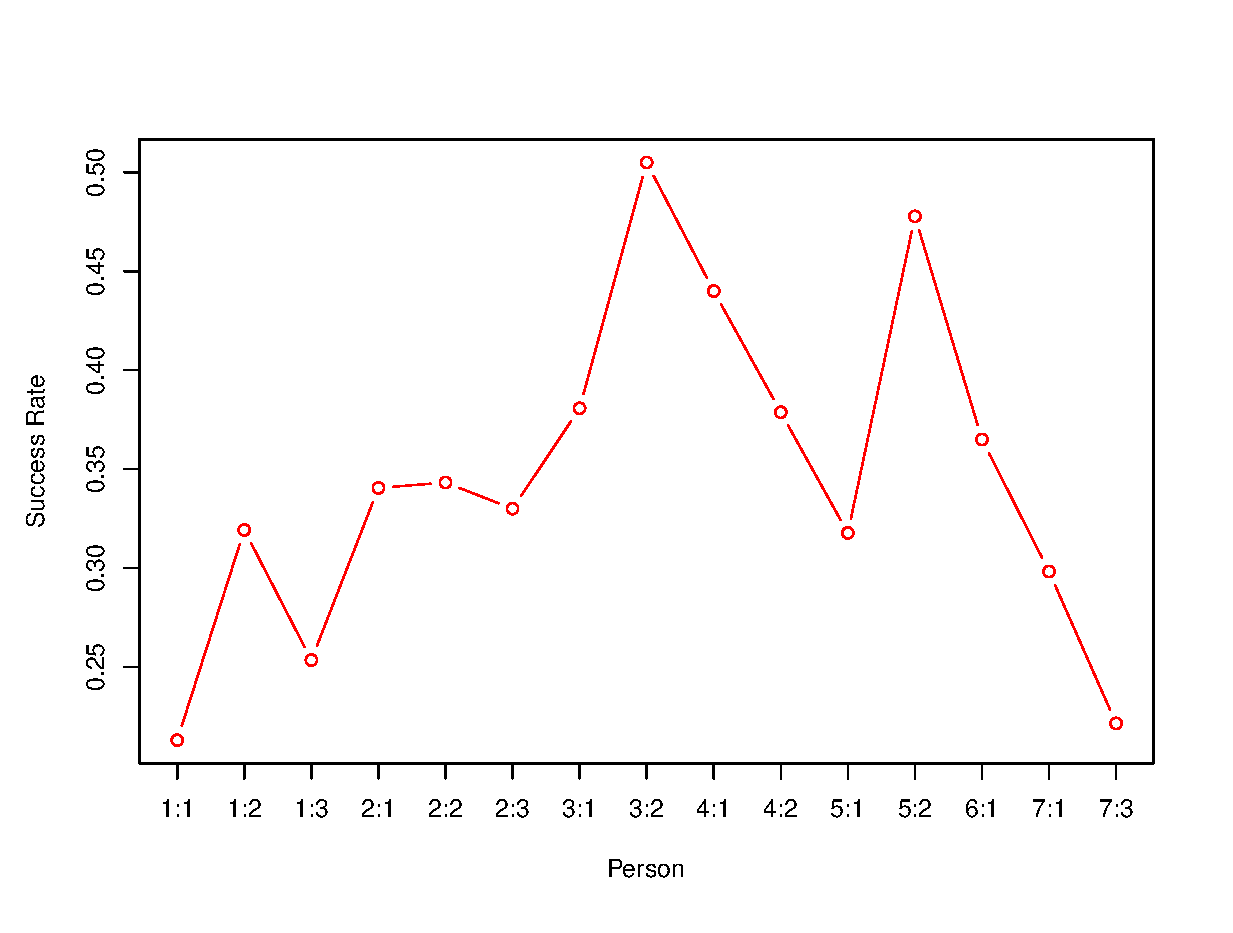
\includegraphics[width = \textwidth]{graphics/graph_baye_comparison}
\caption{Comparison of Naive Bayes for one person with the rest of the class.
Where bins is 50 and PCA is 50\%. The mean success rate is 34.6\%.}
\label{fig:comp_naiveBayes}
\end{figure}

From here it can be seen that this method performs rather bad when testing on the whole class.
With a mean success of 34.6\% for the Naive Bayes, the chance of detecting a decimal correctly is considerably worse than any other previous method  encountered and hence not recommended.

A confusion matrix is also given in table \ref{tb:confus_bayes}.
This is made under same circumstances as figure \ref{fig:comp_naiveBayes} with the test person set to G3M2.

\begin{table}[H]
\centering
	\begin{subtable}{0.75\textwidth}
        \centering
        
\begin{tikzpicture}
            \node at (0,0) {\Large Actual Class}; 
        \end{tikzpicture}
    \end{subtable}
    
    \begin{subtable}{0.05\textwidth}
        \flushright
        
\begin{tikzpicture}
            \node[rotate=90] {\Large Predicted Class};
        \end{tikzpicture}
    \end{subtable}
    \begin{subtable}{0.7\textwidth}
            \centering
%            {\scriptsize
                \begin{tabular}{l|*{10}{c}}
                    &0	& 1	& 2	& 3	& 4	& 5	& 6	& 7	& 8	& 9 \\
\hline
0	& 311	& 8	& 17	& 0	& 1	& 57	& 15	& 13	& 4	& 4 \\
1	& 13	& 247	& 58	& 19	& 19	& 17	& 9	& 37	& 33	& 41 \\
2	& 7	& 5	& 116	& 8	& 0	& 5	& 14	& 32	& 33	& 0 \\
3	& 2	& 18	& 3	& 106	& 0	& 2	& 11	& 50	& 22	& 3 \\
4	& 15	& 15	& 12	& 26	& 323	& 37	& 47	& 92	& 3	& 73 \\
5	& 8	& 4	& 3	& 16	& 0	& 81	& 2	& 0	& 10	& 10 \\
6	& 12	& 38	& 76	& 42	& 5	& 98	& 260	& 5	& 39	& 9 \\
7	& 0	& 1	& 1	& 2	& 0	& 10	& 0	& 109	& 1	& 0 \\
8	& 25	& 45	& 111	& 150	& 0	& 59	& 27	& 15	& 218	& 11 \\
9	& 7	& 19	& 3	& 31	& 52	& 34	& 15	& 47	& 37	& 249 \\

                \end{tabular}
%            }
    \end{subtable}
    \caption{Confusion matrix for Naive Bayes.
    Where bins is 50 and PCA is 50\%. The total success is 50.5\%.}
    \label{tb:confus_bayes}
\end{table}

The data from the confusion matrix in table \ref{tb:confus_bayes} is used to group the ten different decimals into three different groups depending on how well they are detected.
These are seen in table \ref{tab:dec_eval_confus}.

\begin{table}[H]
\centering
\begin{tabular}{|l|c|}
\hline
Group & Decimal \\ \hline
Good ($\geq$ 75\%) & 0, 4 \\ \hline
Intermediate (50\% to 75\%) & 1, 6, 8, 9 \\ \hline
Bad ($\leq$ 50\%) & 2, 3, 5, 7 \\ \hline
\end{tabular}
\caption{Decimal evaluation of confusion matrix in table \ref{tb:confus_bayes}.}
\label{tab:dec_eval_confus}
\end{table}

As can be seen in table \ref{tab:dec_eval_confus}, then the detection of 0 and 4 is quite good, but there is a large amount of miss detected numbers.
The 2's and 3's are often confused with the 8 and the 5 is in many cases confused with the 6.
It can furthermore be seen that the classes 5 and 7 are rarely used to describe a prediction.
Why this is so could be due to their close resemblance to the other classes such as 6 in the case of 5.